% Gemini theme
% https://github.com/anishathalye/gemini

\documentclass[final]{beamer}

% ====================
% Packages
% ====================

\usepackage[T1]{fontenc}
\usepackage{lmodern}
% 60in x  36in
% scale=1.2 corresponds to 
% - body text about 29pt
% - header text about 35pt
% - caption text about 25pt
\usepackage[size=custom,width=152.4,height=91.44,scale=1.2]{beamerposter} 
\usetheme{gemini}
\usecolortheme{rice}
\usepackage{graphicx}
\usepackage{booktabs}
\usepackage{tikz}
\usepackage{pgfplots}
\pgfplotsset{compat=1.14}
\usepackage{anyfontsize}
\usepackage{wrapfig}
\usepackage{caption}

\usepackage{algorithm}
\usepackage[indLines=false]{algpseudocodex}

% Macros
\newcommand{\gr}{\mathrm{gr}}
\newcommand{\defeq}{:=}
\newcommand{\eqdef}{=:}
\newcommand{\relu}{\sigma}
\newcommand{\littleo}{o}
\newcommand{\email}[1]{\texttt{#1}}
\renewcommand{\restriction}{|}
\def\Lambdamap{X}
\newcommand{\isdnet}{ISDnet}
\newcommand{\ODESolve}{\texttt{ODESolve}}
\newcommand{\SANN}{\texttt{SANN}}
\newcommand{\MAtt}{\mathrm{MAtt}}
\newcommand{\Att}{\mathrm{Att}}
\newcommand{\SoftMax}{\mathrm{SoftMax}}
\newcommand{\SArgMax}{\mathrm{SArgMax}}
\newcommand{\saxp}{\mathrm{saxp}}
\newcommand{\LayerNorm}{\mathrm{LayerNorm}}

% ====================
% Lengths
% ====================

% If you have N columns, choose \sepwidth and \colwidth such that
% (N+1)*\sepwidth + N*\colwidth = \paperwidth
\newlength{\sepwidth}
\newlength{\lrcolwidth}
\newlength{\mcolwidth}


\setlength{\sepwidth}{0.025\paperwidth}

% Equispaced
\setlength{\lrcolwidth}{0.3\paperwidth}
\setlength{\mcolwidth}{0.3\paperwidth}

% Larger middle column
% \setlength{\lrcolwidth}{0.25\paperwidth}
% \setlength{\mcolwidth}{0.4\paperwidth}

\newcommand{\separatorcolumn}{\begin{column}{\sepwidth}\end{column}}

% ====================
% Title
% ====================

\title{Semialgebraic Neural Networks: From roots to representations}

\author{S. David Mis \inst{1} \and Matti Lassas \inst{2} \and Maarten V. de Hoop \inst{1}}

\institute[shortinst]{\inst{1} Rice University \samelineand \inst{2} University of Helsinki}

% ====================
% Footer (optional)
% ====================

\footercontent{
  \hfill
  \begin{minipage}[c]{3cm}
    
\includegraphics[height=2cm]{logo_ICLR.pdf}
  \end{minipage}
  \begin{minipage}[c]{0.1\textwidth}
    ICLR 2025, Singapore
  \end{minipage}
  \hfill
  \href{mailto:david.mis@rice.edu}{david.mis@rice.edu}}
% (can be left out to remove footer)

% ====================
% Logo (optional)
% ====================

% use this to include logos on the left and/or right side of the header:
% % Stacked vertically
% \logoleft{%
%   \begin{minipage}[c]{10cm}%
%     \phantom{\quad\quad}\includegraphics[height=3cm]{logo_rice.pdf} \\[1cm]
%     \includegraphics[height=4cm]{logo_helsinki_horiz.pdf}
%   \end{minipage}}
% Side-by-side
\logoleft{
  \begin{minipage}[c]{30cm}
  \raisebox{1cm}{\includegraphics[height=4cm]{logo_rice.pdf}}
  \hspace{1cm}
  \includegraphics[height=6cm]{logo_helsinki.pdf}
  \end{minipage}
}
\logoright{\includegraphics[height=7cm]{qr-code.pdf}}


% ====================
% Body
% ====================

\begin{document}

\begin{frame}[t]
\begin{columns}[t]
\separatorcolumn

\begin{column}{\lrcolwidth}

  \begin{exampleblock}{Abstract}
    Many numerical algorithms in scientific computing---particularly in areas like numerical linear algebra, PDE simulation, and inverse problems---produce outputs that can be represented by semialgebraic functions; that is, the graph of the computed function can be described by finitely many polynomial equalities and inequalities. 
    In this work, we introduce Semialgebraic Neural Networks (SANNs), a neural network architecture capable of representing any bounded semialgebraic function, and computing such functions up to the accuracy of a numerical ODE solver chosen by the programmer.
    Conceptually, we encode the graph of the learned function as the kernel of a piecewise polynomial selected from a class of functions whose roots can be evaluated using a particular homotopy continuation method.
    We show by construction that the SANN architecture is able to execute this continuation method, thus evaluating the learned semialgebraic function.
    Furthermore, the architecture can exactly represent even discontinuous semialgebraic functions by executing a continuation method on each connected component of the target function.
    Lastly, we provide example applications of these networks and show they can be trained with traditional deep-learning techniques.
  \end{exampleblock}

  \begin{block}{Background}
    \begin{itemize}
      \item A function is \textbf{semialgebraic} if its graph is defined by polynomial equalities and inequalities; equivalently, if it can be computed by finitely many operations $+$, $-$, $\times$, $\div$, $\sqrt[n]{\cdot}$, $\texttt{if}$ with polynomial decision boundaries. Examples: Piecewise polynomial and rational functions, solving linear/polynomial systems, polynomial optimization. (See eg. \cite{bochnakRealAlgebraicGeometry1998})
      \item The \textbf{inf-sup definable (ISD)} functions are those that can be computed by combining polynomials with $\max$ and $\min$ operations (equivalently, ReLU activations). The \emph{Pierce--Birkhoff conjecture} states all piecewise polynomials are ISD functions \cite{mahePierceBirkhoffConjecture1984}. ISD functions are computable by \textbf{Matrix-Recurrent Neural Networks (MRNNs)} \cite{dehoopDeepLearningArchitectures2022}.
      \item A \textbf{homotopy continuation method} is a \emph{globally convergent} technique for numerical root-finding. Roots of a difficult function $G$ are found by constructing a homotopy from a simpler function $G_0$; roots of $G_0$ are transformed into roots of $G$ by solving an ODE \cite{chenHomotopyContinuationMethod2015}.
    \end{itemize}
  \end{block}

  \begin{block}{SANN representation theorem}

    % \begin{beamercolorbox}[colsep*=0ex,dp=2ex]{block alerted title}
      \textbf{Theorem:} Every bounded (possibly discontinuous) semialgebraic function is representable by a SANN.
    % \end{beamercolorbox}

    \emph{Proof (continuous case).} Given a continuous semialgebraic function $F: \mathbb{R}^{m} \ni x \mapsto F(x) \in \mathbb{R}^n$:

    \begin{columns}[t]
      \begin{column}{0.19\textwidth}
        \vspace{2cm}
        \begin{figure}[t]
          \centering
          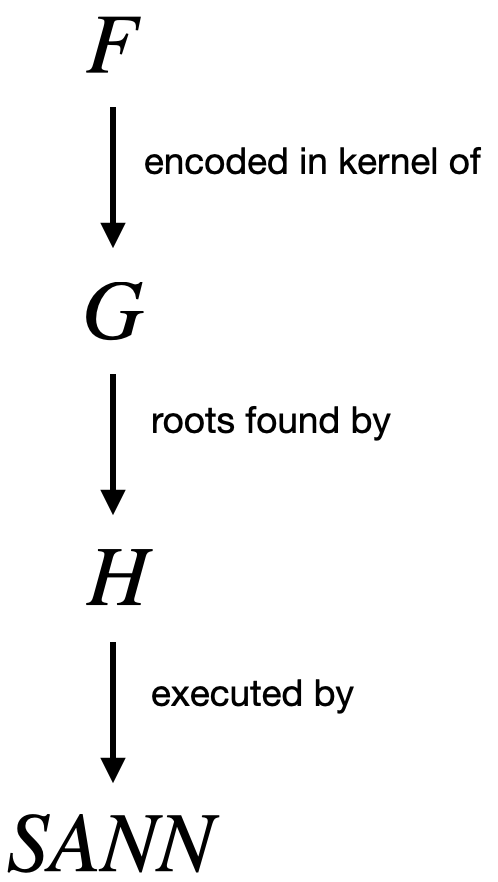
\includegraphics[width=\textwidth]{images/overview.png}       
        \end{figure}
      \end{column}
      \begin{column}{0.6\textwidth}

          % \begin{wrapfigure}{r}{0.2\textwidth}
          %   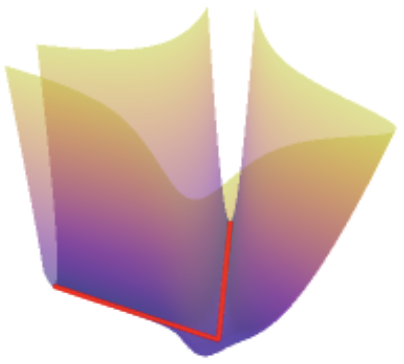
\includegraphics[width=0.9\linewidth]{images/ker_graph.png} 
          %   % \caption*{Semialgebraic $F(x) = |x|$ as the kernel of an ISD function $G$.}
          % \end{wrapfigure}

          \textbf{Step 1}: Construct differentiable ISD $G: \mathbb{R}^{m+n} \to \mathbb{R}^n$ such that the kernel of $G$ is the graph of $F$; ie. $G(x, y) = 0 \Leftrightarrow F(x) = y$.

          \vspace{1cm}
          \textbf{Step 2}: Devise a homotopy continuation method $H: \mathbb{R}^{m+n+1} \to \mathbb{R}^n$  to compute the roots of $G$. We require
          \begin{equation*}
            H(x, y, 0) = G_0(x, y) \text{ and } H(x, y, 1) = G(x, y)
          \end{equation*}
          where for every $x$, it is easy to find $y$ such that $G_0(x, y) = 0$.

          We use the family of ``straight-line'' homotopies
          \begin{equation*}
            H (x, y, t) \defeq (1-t) y + t \big( g(x,y) + G(x,y) \big)
          \end{equation*}
          with $g$ constructed to ensure that for all $x$, there is a \\ smooth curve in the kernel of $H$ that contains $(x, y, 1)$\\ and transversally intersects $t=0$.

          \vspace{1cm}
          \textbf{Step 3}: Design Semialgebraic Neural Networks (SANNs) capable of executing the root-finding method by following the curve in the kernel defined in step 2.
      \end{column}
      
      \begin{column}{0.19\textwidth}
        \vspace{2cm}
        \begin{figure}[t!]
          \centering
          \vspace{-3cm}
          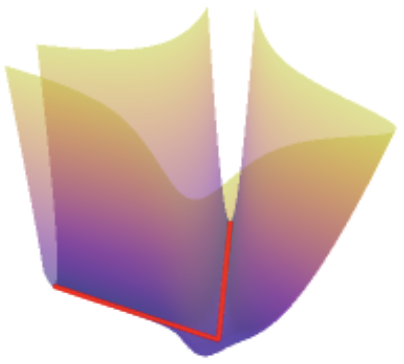
\includegraphics[width=0.9\linewidth]{images/ker_graph.png} 
          % \caption*{Semialgebraic $F(x) = |x|$ as the kernel of an ISD function $G$.}        
        \end{figure}
        \vspace{4cm}
        \begin{figure}[t]
          \hspace*{-4cm} 
          \centering
          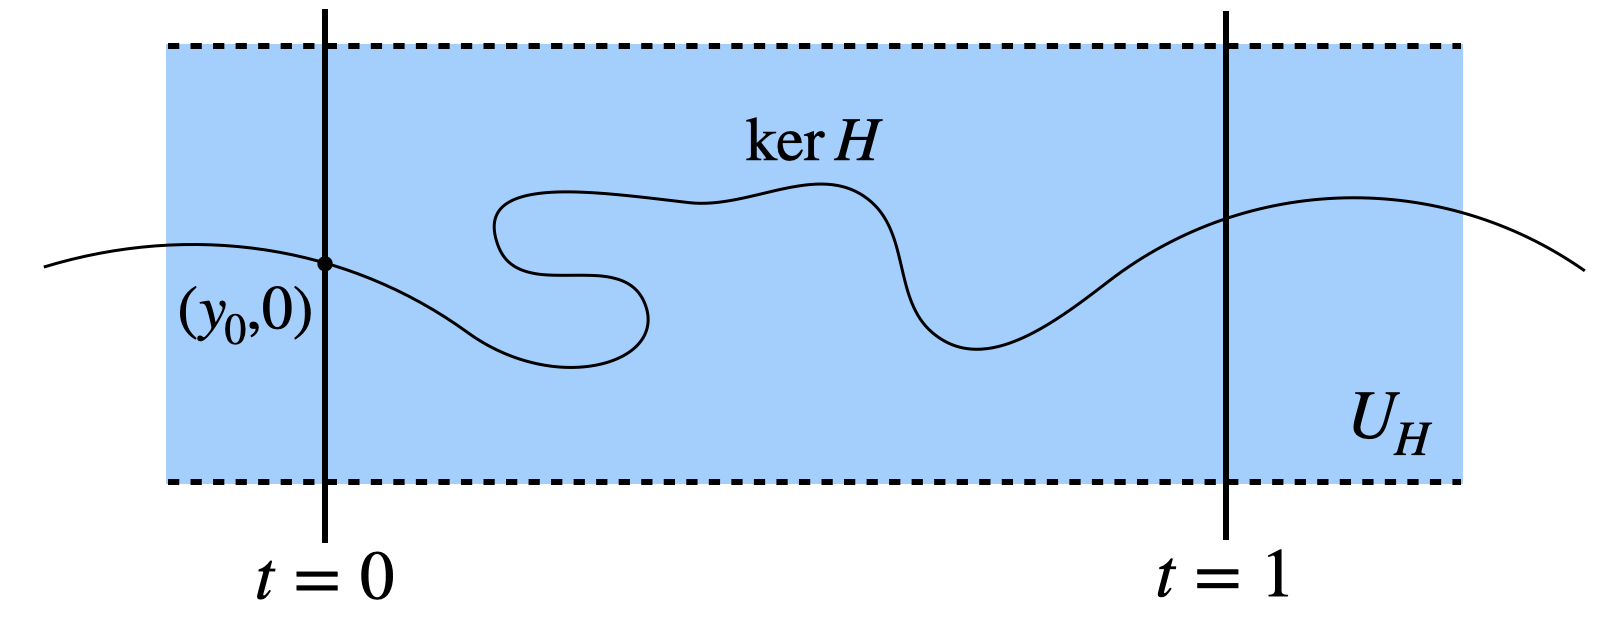
\includegraphics[width=1.5\linewidth]{images/krantz_and_parks_curve.png}        
        \end{figure}
      \end{column}
    \end{columns}
    \vspace{1cm}
    \textbf{Extension to discontinuous functions}:
    By using singular matrices in a controlled way, we can extend the constructions in the representation theorem to work even for discontinuous semialgebraic functions.
  \end{block}
\end{column}

\separatorcolumn

\begin{column}{\mcolwidth}

  \begin{alertblock}{Main results: We show}
    \begin{enumerate}
      \item Every bounded (possibly discontinuous) semialgebraic function $F$ is the solution of some ODE initial value problem corresponding to a \textbf{homotopy continuation method} for root finding.
      % \item \textbf{Representation theorem:} Every bounded (possibly discontinuous) semialgebraic function $F$ is representable as a \textbf{Semialgebraic Neural Networks (SANNs)} that numerically evaluates its associated ODE.
      \item \textbf{Semialgebraic Neural Networks (SANNs)} can learn $F$ by learning its associated ODE. \textbf{Every bounded (possibly discontinuous) semialgebraic function $F$ can be represented by a SANN.}
    \end{enumerate}
\end{alertblock}

  \begin{figure}
    \centering
    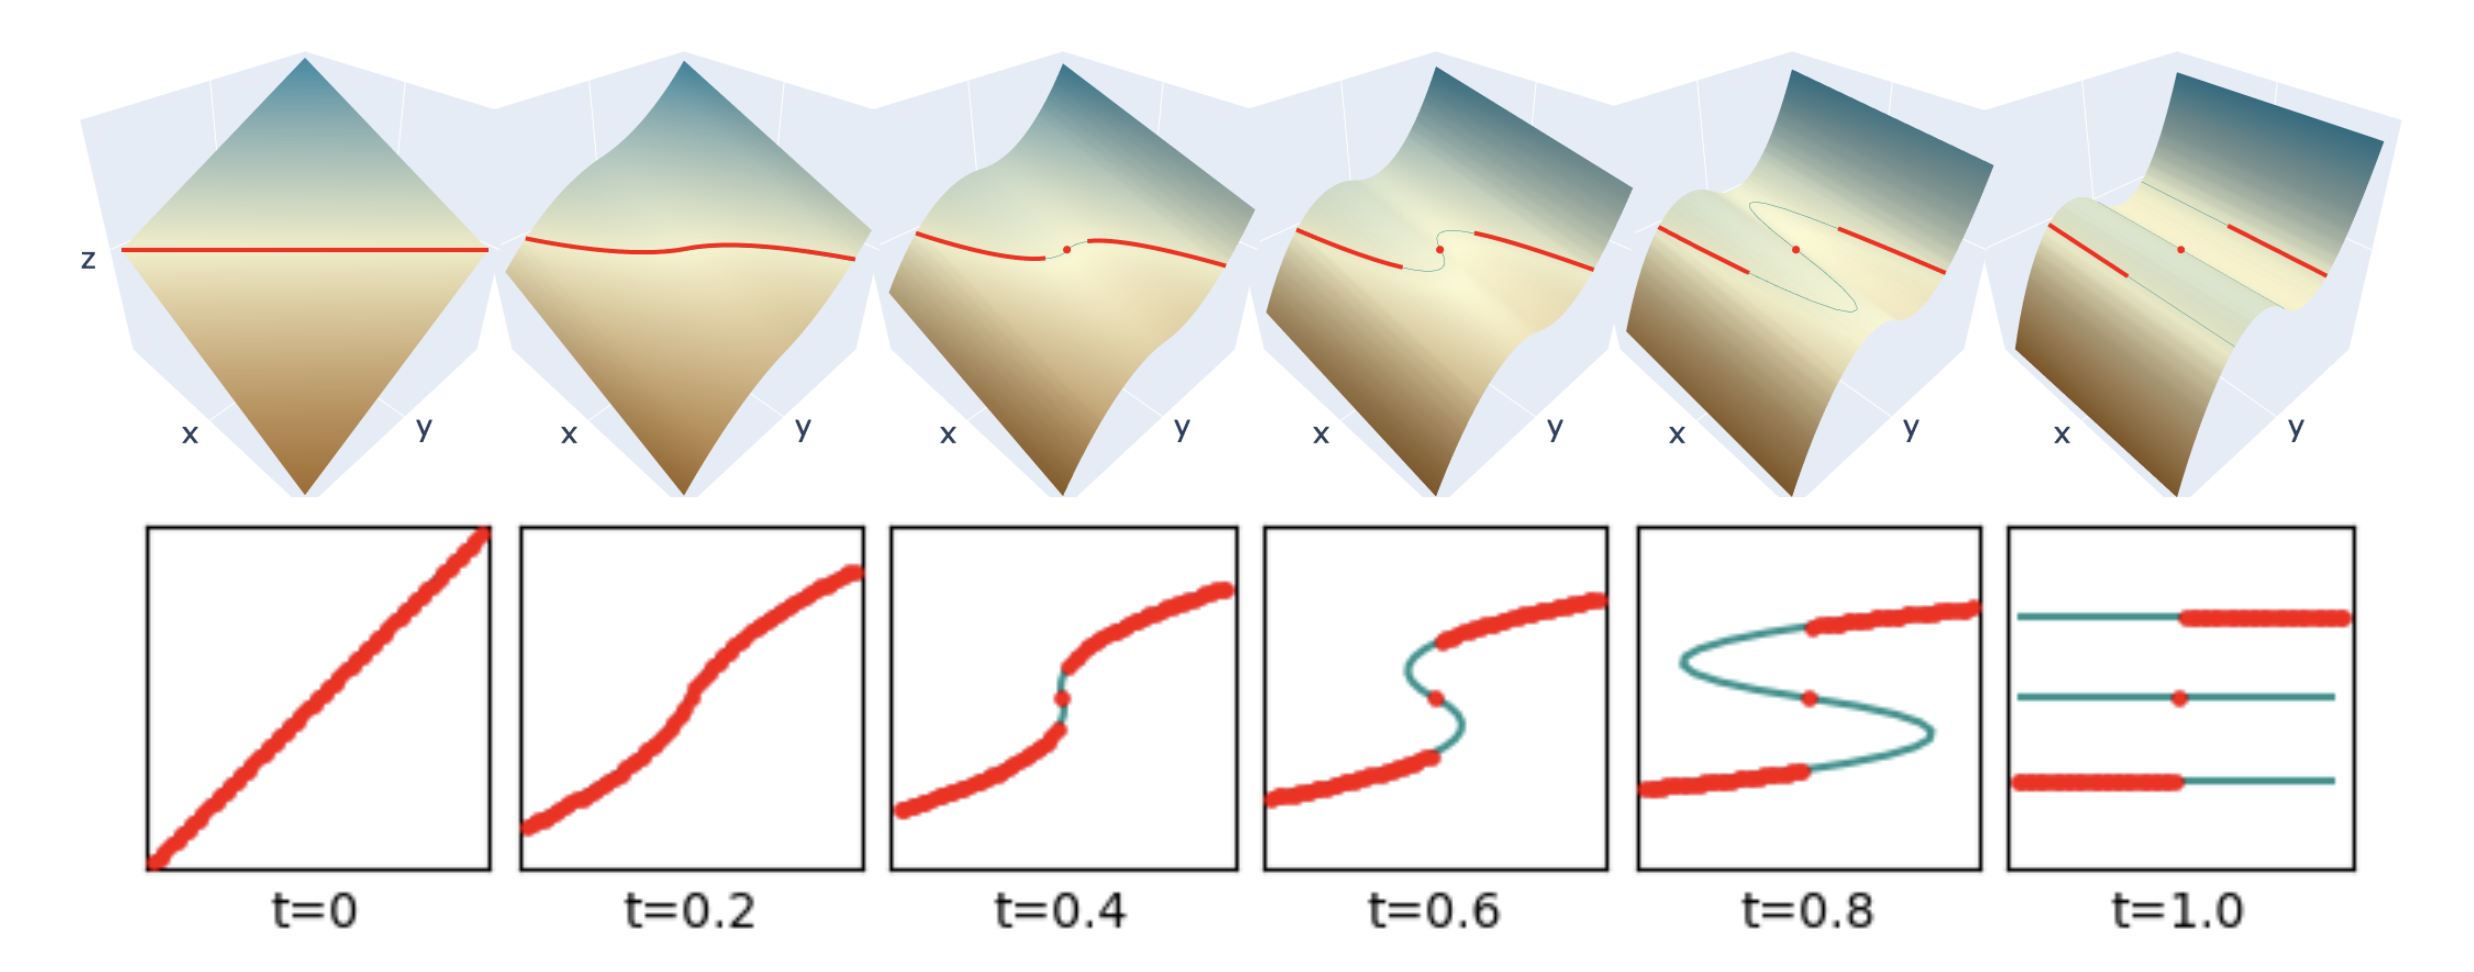
\includegraphics[width=\linewidth]{images/heaviside_homotopy.png}
    \caption*{
      Computing the Heaviside step function $F$ (plotted in red) using a homotopy method. 
      The graph of $F$ is a subset of the kernel of a higher-dimensional piecewise polynomial $G$.
      In the upper row, we plot the surface of a homotopy $H$ such that $H(x,y,0)=0$ is trivial to solve (upper left), and $H(x,y,1)=G$ (upper right).
      The kernel of $H$ is shown with a green line (red points are also on top of the green line).
      The bottom row shows the projection of $H$ onto the $xy$-plane.
      We compute $F(x)=y$ by following the kernel of $H$ from time $t=0$ to $t=1$, keeping $x$ fixed.
      Although the kernel of $G$ contains points outside the graph of $F$ (the visible parts of the green lines), these points are never encountered when computing $F$ by following the homotopy.
      This process captures the discontinuity exactly, including the isolated point at $(0,0)$. 
    }
  \end{figure}

  % \begin{columns}
  %   \begin{column}{0.1875\paperwidth}
  %   \end{column}
  %   \separatorcolumn
  %   \begin{column}{0.1875\paperwidth}
  %   \end{column}
  % \end{columns}

  \begin{block}{ODE system}
    % Every bounded semialgebraic function is the solution to an ODE of the form:
    % \begin{align}
    %   \dot z(s)&=\hbox{clamp-sol}(M(x,z(s),s),b(x,z(s),s)), \label{ODE-alt} \\
    %   z(0)&=0. \label{ODE-alt2}
    % \end{align}
    % Matrix $M(x,z,s)$ and vector $b(x,z,s)$ are the output of an ISD network ${\mathcal N}(x,z,s)$. The function $\textrm{clamp-sol}$ is defined 
    % \begin{equation}
    % \textrm{clamp-sol}(M,b) \defeq \begin{cases}
    %         \hbox{clamp}(M^{-1}b,-c_{\max},c_{\max}) & \text{if $M$ is invertible} \\
    %         0 & \text{otherwise.}
    %     \end{cases}
    % \end{equation}
    % The function ``$\textrm{clamp}$'' operates component-wise on each element of a vector, and is defined
    % \begin{equation}
    %     \textrm{clamp}(a, low, high) \defeq \begin{cases} a, & a \in [low, high] \\
    %     low, & a < low \\
    %     high & a > high.
    %     \end{cases}
    % \end{equation}

    % The ODE system is numerically evaluated using any scheme chosen by the programmer; we use the Forward Euler method
    % \begin{align}\label{ODE-alt disc}
    %   z_{j+1} &= \textrm{ODE-step}\left(\dot{z}_j, z_j, \frac{j}{N} \right) \defeq z_j +\frac{1}{N} \dot{z}_j
    % \end{align}

    SANNs numerically evaluate the solution of an
    ordinary differential equation
    by setting $z_0=0$ and defining 
    for $j=0,1,\dots,N-1$,
    \begin{align}\label{ODE-alt disc}
        z_{j+1} &= \textrm{ODE-step}\left(\dot{z}_j, z_j, \frac{j}{N} \right) \defeq z_j +\frac{1}{N} \dot{z}_j
    \end{align} 
    where
    \begin{align}
        \dot z_j&=\textrm{clamp-sol} \left( M \Big(x,z_j,\frac jN \Big), b\Big(x,z_j,\frac jN \Big) \right). \label{ODE-alt discrete}
    \end{align}
    Matrix $M(x,z,s)$ and vector $b(x,z,s)$ are the output of MRNNs. The function $\textrm{clamp-sol}$ is defined 
    \begin{equation}
    \textrm{clamp-sol}(M,b) \defeq \begin{cases}
            \hbox{clamp}(M^{-1}b,-c_{\max},c_{\max}) & \text{if $M$ is invertible} \\
            0 & \text{otherwise.}
        \end{cases}
    \end{equation}
    The function ``$\textrm{clamp}$'' operates component-wise on each element of a vector, and is defined
    \begin{equation}
        \textrm{clamp}(a, low, high) \defeq \begin{cases} a, & a \in [low, high] \\
        low, & a < low \\
        high & a > high.
        \end{cases}
    \end{equation}
    These functions guarantee the iteration (\ref{ODE-alt discrete}) is well-defined even when $\mathcal{N}$ produces singular or nearly-singular output matrices $M$. 
    Lastly, $\Pi$ projects onto the first $n$ components of its input.

    The iteration (\ref{ODE-alt discrete})
    is the  Euler finite-difference scheme that approximates 
    the solution of the ODE
    \begin{align}
        \dot z(s)&=\hbox{clamp-sol}(M(x,z(s),s),b(x,z(s),s)), \label{ODE-alt} \\
        z(0)&=0. \label{ODE-alt2}
    \end{align}
    As $N\to \infty$, the output of the finite difference scheme converges
    to the solution of the ODE.
    These limit functions are of the form $f^{lim}_{\mathcal{N},c_{\text{max}}}:x\mapsto \Pi z(1)$ that are defined
    by the ODE (\ref{ODE-alt})--(\ref{ODE-alt2}). We call these functions as the limit functions of 
    SANNs and denote those by $SANN^{lim}(\mathcal{N}, \cdot, c_{\max})$.
    We note that the forward-Euler definition for ODE-step used in (\ref{ODE-alt disc}) can be replaced with other numerical solvers, such as Runge-Kutta methods.

  \end{block}
\end{column}

\separatorcolumn

\begin{column}{\lrcolwidth}

  \begin{block}{Neural network architecture}
    \begin{columns}
      \begin{column}{0.7\textwidth}
        \begin{algorithm}[H]
          \caption{Evaluating a SANN}
          \label{alg-sann}
          \begin{algorithmic}[1]
              \Require $\mathcal{N} \in \isdnet(m, n, k)$ \\
              $x \in \mathbb{R}^m$ \\
              $c_{\max} \in \mathbb{R}_{\ge 0}$
              
              \Function {\SANN}{$\mathcal{N}$, $x$, $c_{\max}$} 
                  \Function{$\dot{z}$}{$z$, $s$}
                      \State $(M, b) \leftarrow \mathcal{N}(x, z, s)$ \label{line-Mb}
                      \If {$M$ is singular} \label{line-M-singular-1}
                          \State \Return $0$ \label{line-M-singular-2}
                      \Else 
                          \State \Return \texttt{clamp}$(M^{-1} b$, $-c_{\max}, c_{\max})$ \label{line-clamp}
                      \EndIf
                  \EndFunction
                  \State $(y, t) \leftarrow \ODESolve( \dot{z}, (0, 0) )$ \label{line-ODESolve}
                  \State \Return $y$
              \EndFunction
            \end{algorithmic}
          \end{algorithm}

          Architecture diagram for a SANN. The SANN outputs $y$ as a semialgebraic function of input $x$. Vectors $z_j$ are the current values of an ODE at timestep $j$. The time-derivative $\dot{z}_j$ is computed using a neural network $\mathcal{N}$ capable of computing ISD piecewise polynomials. $\mathcal{N}$ accepts the current ODE state $(z_j, j/N)$, as well as recurrent input $x$. The output of $\mathcal{N}$ is a matrix $M$ and vector $b$, from which $\dot{z}_j$ is computed using $\hbox{clamp-sol}(M, b)$ ($\dot{z}_i = M^{-1} b$ in the common case). $\hbox{ODE-step}$ is a single update of a numerical ODE solver. Finally, $\Pi$ is a projection operation such that $y$ is the first $n$ components of $z$. 
      \end{column}
      \begin{column}{0.3\textwidth}

        % 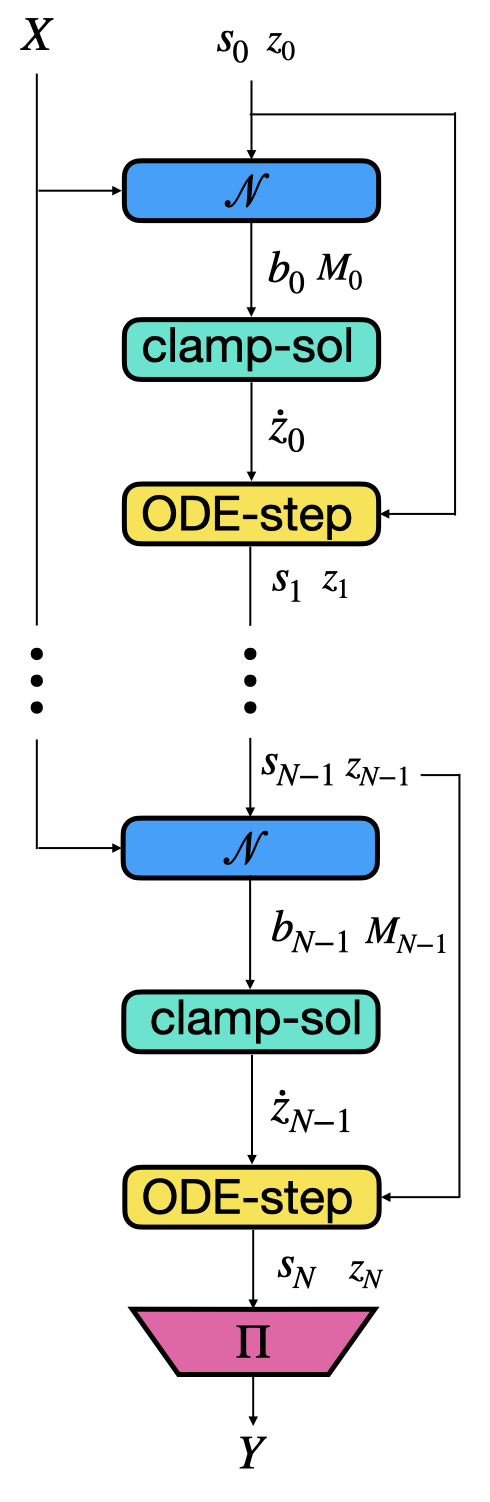
\includegraphics[width=0.8\linewidth]{images/architecture_vert.001.png}

        \begin{figure}[t]
          \centering
          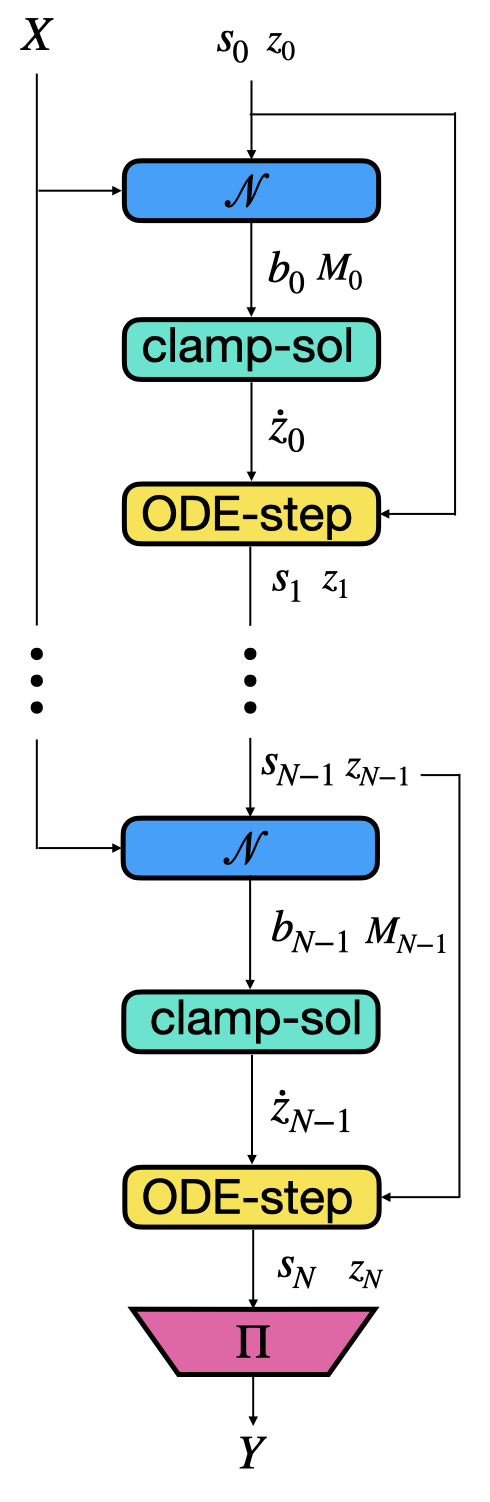
\includegraphics[width=0.8\linewidth]{images/architecture_vert.001.png}         
        \end{figure}
      \end{column}
    \end{columns}

  
    % \begin{figure}[t]
    % \centering
    %   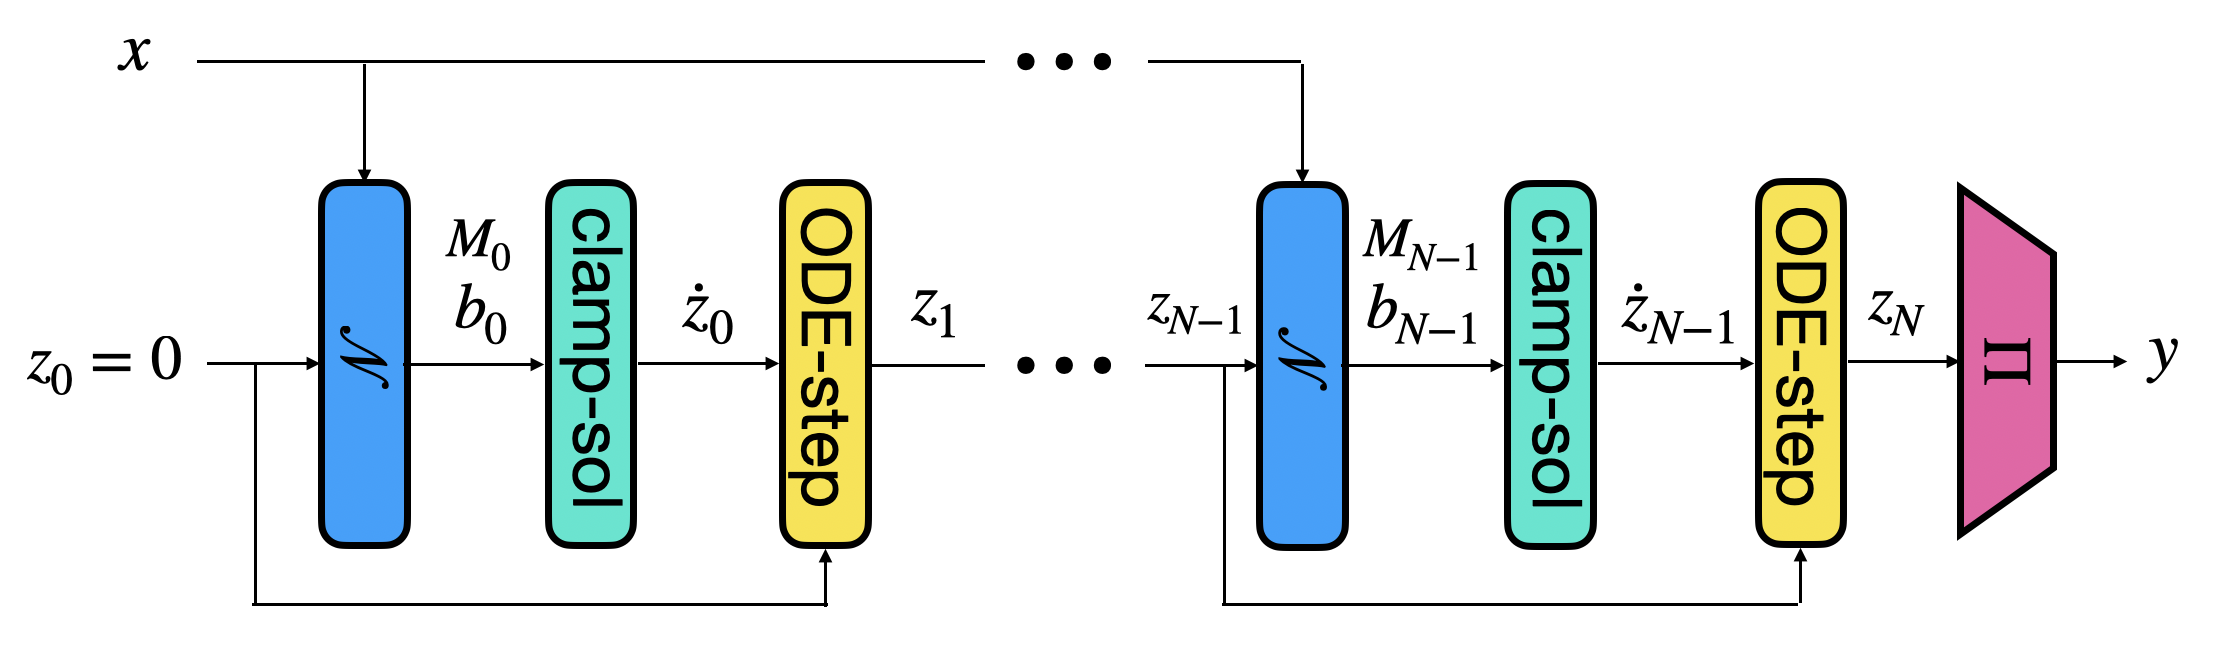
\includegraphics[width=0.8\linewidth]{images/architecture.png}
    %   \caption{

    %   }
    % \end{figure}

    
  \end{block}

  \begin{block}{Numerical example: Matrix inversion}
    Figure: handcrafted example. Table: trained on data.
    \begin{figure}[h]
      \centering
      \begin{minipage}[c]{0.49\textwidth}
          \includegraphics[width=\linewidth]{images/jacobi_sann50.pdf}
      \end{minipage} \hfill
      \begin{minipage}[c]{0.5\textwidth}
          \caption*{(Left) Trajectories of a SANN that solves linear systems to machine precision. Given a matrix $X \in \mathbb{R}^{50 \times 50}$ and vector $b \in \mathbb{R}^{50}$, the network produces a vector $y \in \mathbb{R}^{50}$ such that $Xy = b$. Each line shows the trajectory of the output $y$ for a given input pair $(X, g)$ as the SANN's ODE is iteratively solved. At each timestep, the network performs a single Jacobi iteration update. The output of the network exactly matches the output of $100$ steps of Jacobi iteration.}
          \label{fig:jacobi_sann}
          \begin{table}[h]
            \centering
            \begin{tabular}{c|c|c}
              & \# parameters & $\| Xy - g \|_2$ \\ \hline
              MLP & $306,140$ & $0.166$ \\ \hline
              SANN & $\mathbf{291,720}$ & $\mathbf{0.101}$
            \end{tabular}
            \caption*{(Table) Results of training a SANN and feed-forward neural network to solve linear systems. Given a $10 \times 10$ matrix $X$ and vector $g$, the networks output $y$ such that $Xy \approx g$.}
          \end{table}
      \end{minipage}
    \end{figure}

  \end{block}

  \begin{block}{References}

    \nocite{*}
    \footnotesize{\bibliographystyle{plain}\bibliography{poster}}

  \end{block}

\end{column}

\separatorcolumn
\end{columns}
\end{frame}

\end{document}
